\documentclass[../main.tex]{subfiles}

\section{Contexto} \label{section:contexto-intro}
%Orientacion y navegación muy antiguos (primeros mapas). Primeros sistemas 
La navegación y posicionamiento en tierra se ha practicado durante mucho tiempo. Los primeros sistemas radio surgen en los años 40, cuando el sistema LORAN (\emph{LOng-RANge navigation system}) fue introducido. Este sistema permitía a los barcos triangular su posición usando señales radio desde estaciones LORAN terrestres. El primer satélite, Sputnik \cite{hofmann.2007gnss}, fue lanzado en 1957 y no mucho después los científicos contemplaron por primera vez la opción de trabajar desde una órbita satelital conocida para determinar una posición en la tierra. El primer sistema satelital fue el sistema Transit \cite{hofmann.2007gnss}, en los años 1960, que no se considera un sistema de navegación global por satélite, (GNSS, \emph{Global Navigation Satellite System}), pues no ofrecía cobertura global las 24 horas. \\
El concepto GNSS surge posteriormente en los años 70, con el desarrollo del sistema estadounidense NAVSTAR-GPS (\emph{Navigation System Time And Ranging-Global Positioning System}) \cite{hofmann.2007gnss}. Sin embargo, a pesar de tener cobertura mundial, no era ``global'' como indica su nombre, ya que era un sistema exclusivamente de uso militar. Así pues, es en los noventa cuando se permite su uso civil y múltiples países alcanzan acuerdos con el Gobierno estadounidense para adherirse al uso del sistema. \\
Surge así la necesidad para las demás potencias de tener su propio sistema de navegación por satélite. Europa desarrolla Galileo y Rusia lanza GLONASS como sistemas globales, mientras China plantea Beidou, la India IRNSS y Japón QZSS como sistemas regionales \cite{hofmann.2007gnss}.  \\
Son muchas y muy diversas las aplicaciones de los GNSS: industria cartográfica y topográfica, minería, navegación autónoma, etc. En la actualidad, vehículos, ya sea en tierra, mar o en aire, utilizan a diario el posicionamiento proporcionado por los sistemas GNSS. \\
Los drones o UAV (\emph{Unmanned Aerial Vehicle}) se han popularizado en los últimos años hasta el punto de formar parte de nuestro día a día con aplicaciones en muchos ámbitos de nuestra vida. Un UAV es un vehículo sin tripulación, reutilizable, capaz de mantener de manera autónoma un nivel de vuelo controlado y sostenido, y propulsado por un motor de explosión, eléctrico o de reacción. \\
Los sistemas GNSS, predominantes en el posicionamiento y localización en exteriores, tiene un mal funcionamiento en interiores debido al bajo nivel de señal disponible. Las señales satelitales no están diseñadas para alcanzar interiores de construcciones, pues las frecuencias utilizadas no pueden penetrar en la mayoría de los materiales de construcción \cite{stone.1997}. Debido a esto, el posicionamiento en interiores (IPS, \emph{Indoor Positioning System}) ha sido un ámbito de mucho interés en investigación y muchos sistemas han sido propuestos en las últimas décadas como solución al problema existente. \\

\section{Problema y motivación} \label{section:probmotiv-intro}
Este estudio se centra en el estudio de los sistemas de posicionamiento en interiores, con especial atención, pero no en exclusiva, al posicionamiento de drones en interiores. Como ya se ha mencionado anteriormente, los drones son cada vez mas usados y las posibilidades existentes para su posicionamiento son muy amplias. En concreto, son los drones de pequeño tamaño (MAVs, \emph{Micro Aerial Vehicles}) los que interesa posicionar. \\
Esta aplicación surge debido a una necesidad para posicionar MAVs de forma no intrusiva y económicamente viable para el público general. Esto viene motivado por el interés de cierto grupo de profesores de la URJC para un posible proyecto y aplicación comercial futura, la cual trataremos en detalle durante el trabajo. Sobre este proyecto surge la duda de que sistema de posicionamiento es el más adecuado utilizar. De esta forma, se plantea realizar un estudio general sobre los sistemas de posicionamiento y una comparativa que permita seleccionar un sistema-solución en función de la aplicación específica. \\
En resumen, lo que se persigue es realizar un estudio de la ciencia de posicionamiento en interiores que permita proponer una solución que posibilite el correcto posicionamiento del problema concreto tratado en este texto. Para ello, se busca desarrollar un modelo comparativo que se pueda aplicar, no solo a la aplicación aquí formulada, sino para cualquier aplicación que necesite un posicionamiento en interiores.

\section{Objetivos} \label{section:objetivos-intro}
Este estudio presenta múltiples objetivos. En primer lugar, se quiere reflejar el estado del arte de los sistemas de posicionamiento en interiores y su taxonomía. El primer objetivo se abordará desarrollando un espectro abstracto de sistemas que se adapte a las tendencias y a las necesidades actuales, representando de una forma sencilla pero completa los sistemas existentes. Para ello, una clasificación será propuesta que permita un correcto análisis de los componentes de un sistema. \\
En segundo lugar, se quiere exponer un método comparativo que permita evaluar diferentes sistemas en función de la aplicación concreta del problema a resolver. Beneficiándose de la taxonomía expuesta previamente, un modelo y un baremo serán sugeridos que permitan confrontar los sistemas valorados como resolución del problema. \\
Por último, sirviéndose de lo desarrollado hasta el momento, se recomendará un sistema solución para el problema contemplado en este trabajo (ver Sección \ref{section:probmotiv-intro}). La solución sugerida será una primera aproximación al sistema completo, pues una solución íntegra escapa al alcance de este trabajo. \\
Así pues, los objetivos principales contemplados en este trabajo son:

\begin{enumerate}
    \item Representación y clasificación de los sistemas de posicionamiento en interiores actuales. 
    \item Desarrollo de un método comparativo que permita seleccionar un sistema según los requisitos de una aplicación concreta.
    \item Aproximación a un sistema solución para la aplicación propuesta.
\end{enumerate}



\section{Estructura de la memoria} \label{section:estructura-intro} 
A continuación, se introduce la estructura de la memoria de este estudio, al igual que los diferentes temas tratados en cada capítulo. \\
En primer lugar, se propone una descripción general con una clasificación de los IPS. Durante el trabajo, se hará distinción entre técnicas y tecnologías (Fig. \ref{fig:ips}), donde el término ``técnica'' se refiere a una herramienta abstracta básica, no necesariamente vinculada a los medios físicos, que podría usarse en varias``tecnologías'' mientras que las``tecnologías'' son formas específicas de usar señales físicas, registradas a través de sensores, como ondas de radio o campos magnéticos, para cumplir los objetivos de un IPS. En un ejercicio de abstracción, se ha obviado la aplicación concreta para el sistema. De esta forma, se ha propuesto un método de división y clasificación independiente a la aplicación del sistema. \\
La clasificación propuesta no es, ni mucho menos, una gran innovación. Muchos autores han propuestos sus propias clasificaciones a lo largo de los años, entre los que queremos destacar a autores como \emph{Hightower y Borriello} \cite{Hightower.2001}, \emph{Liu et al.} \cite{Liu.2007}, \emph{Mautz} \cite{Mautz.2012}, \emph{Brena et al.} \cite{Brena.2017} y \emph{Sakpere et al.} \cite{Sakpere.2017}.
Estos estudios pese a diferir en diversos aspectos de la clasificación propuesta han sentado la base para tendencia actual en la clasificación de sistemas IPS, y sirven para hacerse con una visión global del estado de la ciencia que nos compete. A estos artículos nos referiremos en repetidas ocasiones a lo largo de la memoria. \\

\begin{figure}[ht]
    \centering
    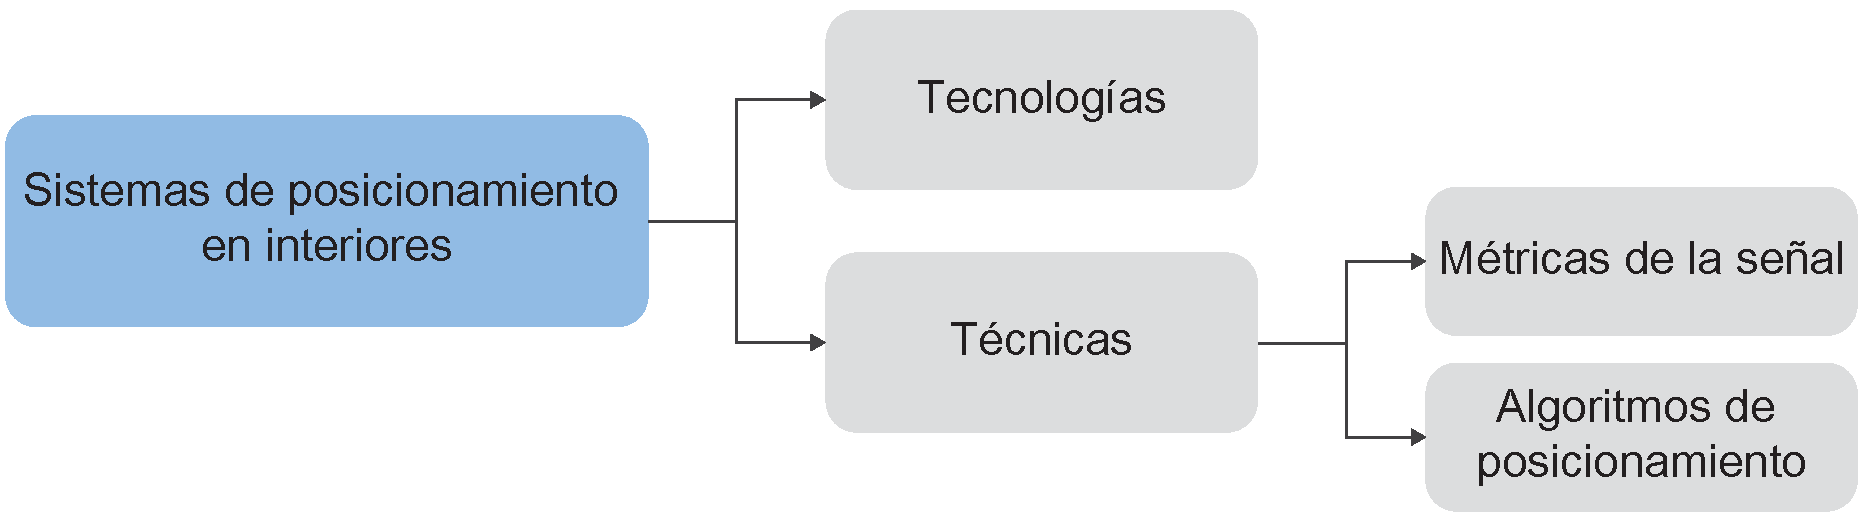
\includegraphics[width=0.8\textwidth]{base.pdf}
    \caption{Esquema que muestra la clasificación de los sistemas IPS seguida.}
    \label{fig:ips}
\end{figure}

En primer lugar, el criterio seguido para esta división ha sido las diferentes herramientas abstractas básicas (\emph{técnicas}) (Cap. \ref{chapter:tecnicas}). Se han utilizado las propiedades físicas de la señal durante la Sección \ref{section:metricas} y los algoritmos o métodos de posicionamiento durante la Sección \ref{section:algoritmos} para diferenciar los sistemas entre sí. Las métricas más relevantes son la directa o física, el ángulo de llegada (AoA), el tiempo de llegada (ToA), el tiempo diferencial de llegada (TDoA) y la intensidad de señal recibida (RSSI). Por otro lado, los algoritmos de posicionamiento más destacables son la multilateración (lateración y angulación), el análisis por proximidad (o detección directa), el análisis del entorno (\emph{fingerprinting}) y la navegación por estima (o navegación inercial, INS). \\
A continuación, el criterio de clasificación se establece en el modo específico de utilizar estas herramientas (\emph{tecnologías}) (Cap. \ref{chapter:tecnologias}). A su vez, se han ligado estas tecnologías con las diferentes técnicas previamente, estableciendo diferentes conexiones entre ambas, pues no son conceptos aislados. Dentro las tecnologías existentes usadas en IPS se incluyen tecnologías como; óptica (infrarrojos (IR), luz visible (VCL) o dispositivos), acústica (ultrasonidos o audible), magnética, de radio-frecuencia (RF) e híbridas.
Algunas tecnologías de RF son Bluetooth, banda ultra-ancha (UWB), red de sensores inalámbricos (WSN), red inalámbrica local (WLAN, IEEE 802.11), identificación por radio-frecuencia (RFID) y comunicación por campo cercano (NFC). \\
En la Figura \ref{fig:integracion} se representa la estructura básica de un sistema de posicionamiento en interiores. En ella se integran las diferentes técnicas y tecnologías para formar un sistema concreto. Con esta figura se intenta esclarecer la función que lleva a cabo cada elemento dentro de un IPS. \\

\begin{figure}[ht]
    \centering
    \includegraphics[width=0.8\textwidth]{integracion.pdf}
    \caption{Estructura típica de un IPS \cite{pahlavan.2002}.}
    \label{fig:integracion}
\end{figure}

La mayoría de sistemas existentes consisten en una solución híbrida, tanto de tecnologías como de técnicas, con el objetivo de cumplir requisitos más elevados de exactitud, precisión, complejidad, escalabilidad, privacidad, seguridad, usabilidad o coste. Estos requisitos son revisados durante el Capítulo \ref{chapter:comparativa} con el objetivo de plantear un marco común de comparación.
Seguidamente, se ha establecido un modelo con estos criterios que permita evaluar las diferentes tecnologías y hallar el sistema que mejor se adapte a un servicio concreto. 
La metodología seguida durante la comparativa, y en general durante este estudio, también es explicada en este capítulo. \\
Por último, durante el Capítulo \ref{chapter:estudio} se ha aplicado la taxonomía presentada, y sobre los resultados obtenidos, se ha aportado un posible sistema solución al problema concreto. La aplicación seleccionada también es explicada durante este capítulo (Sec. \ref{section:aplicacion}). Sobre la solución aportada hay que decir que no se pretende aportar un sistema íntegro con todo lo necesario para su implementación, sino una primera aproximación que permita también entender la metodología aplicada a la comparativa.\\
Finalmente, en el Capitulo \ref{chapter:conclusiones} se exponen las conclusiones extraídas a lo largo del desarrollo del trabajo y se evalúan los objetivos iniciales propuestos. A mayores, se exponen una serie de posible líneas futuras de trabajo que pueden surgir de este estudio.
